\section{Evaluation}

\begin{frame}[t]{Example}
\begin{itemize}
  \item Video frame processing for border detection with two filters.
    \begin{itemize}
      \item Gaussian blur.
      \item Sobel.
    \end{itemize}
  \vfill\pause
  \item Using \textgood{pipeline} pattern:
    \begin{itemize}
      \item S1: Frame reading.
      \item S2: Gaussian blur (may apply \textgood{farm}).
      \item S3: Sobel filter (may apply \textgood{farm}).
      \item S4: Frame writing.
    \end{itemize}
  \vfill\pause
  \item \textenum{Approaches}:
    \begin{itemize}
      \item Manual.
      \item \textmark{GrPPI}.
    \end{itemize}
\end{itemize}
\end{frame}

\begin{frame}{Parallelization effort}
\footnotesize
\begin{tabular}{|c|r|r|r|r|r|}
\hline
Pipeline & \multicolumn{5}{c|}{\centering\let\newline\\ \% LOC increase} \\\cline{2-6}
Composition & \textbf{C++ Threads}  & \textbf{OpenMP} & \textbf{Intel TBB}  & \textbf{Fastflow} & \textbf{GrPPI} \\\hline\hline
\texttt{(\,p\,$|$\,p\,$|$\,p\,$|$\,p\,)} & $+$8.8\,\%   & $+$13.0\,\%  & $+$25.9\,\% & $+$16.5\,\% & $+$1.8\,\% \\
\texttt{(\,p\,$|$\,f\,$|$\,p\,$|$\,p\,)} & $+$59.4\,\%  & $+$62.6\,\%  & $+$25.9\,\% & $+$24.7\,\% & $+$3.1\,\% \\
\texttt{(\,p\,$|$\,p\,$|$\,f\,$|$\,p\,)} & $+$60.0\,\%  & $+$63.9\,\%  & $+$25.9\,\% & $+$24.7\,\% & $+$3.1\,\% \\
\texttt{(\,p\,$|$\,f\,$|$\,f\,$|$\,p\,)} & $+$106.9\,\% & $+$109.4\,\% & $+$25.9\,\% & $+$39.2\,\% & $+$4.4\,\% \\\hline
\end{tabular}
\end{frame}

\begin{frame}{Performance: frames per second}
\includegraphics[height=.85\textheight]{fps.pdf}
\end{frame}

\begin{frame}[t]{Brain MRI (Magnetich Resonance Imaging)}
\begin{columns}
\column{.7\textwidth}
\begin{itemize}
  \item Non intrusive method for getting internal anatomy.
  \item Huge amount of data generated.
  \item Applied to neuro-sciences.
    \begin{itemize}
      \item Bipolar disorder.
      \item Paranoia.
      \item Schizophrenia.
    \end{itemize}
\end{itemize}

\column{.3\textwidth}
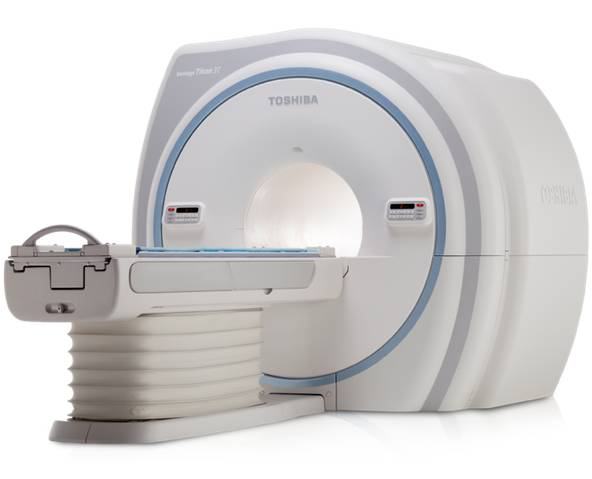
\includegraphics[width=\textwidth]{img/mri-scanner.jpg}
\end{columns}

\vspace{2em}
\begin{itemize}
  \item Identification of fibers and connectivity between areas in brain.
\end{itemize}

\end{frame}

\begin{frame}[t]{Fibbers in brain}
\begin{center}
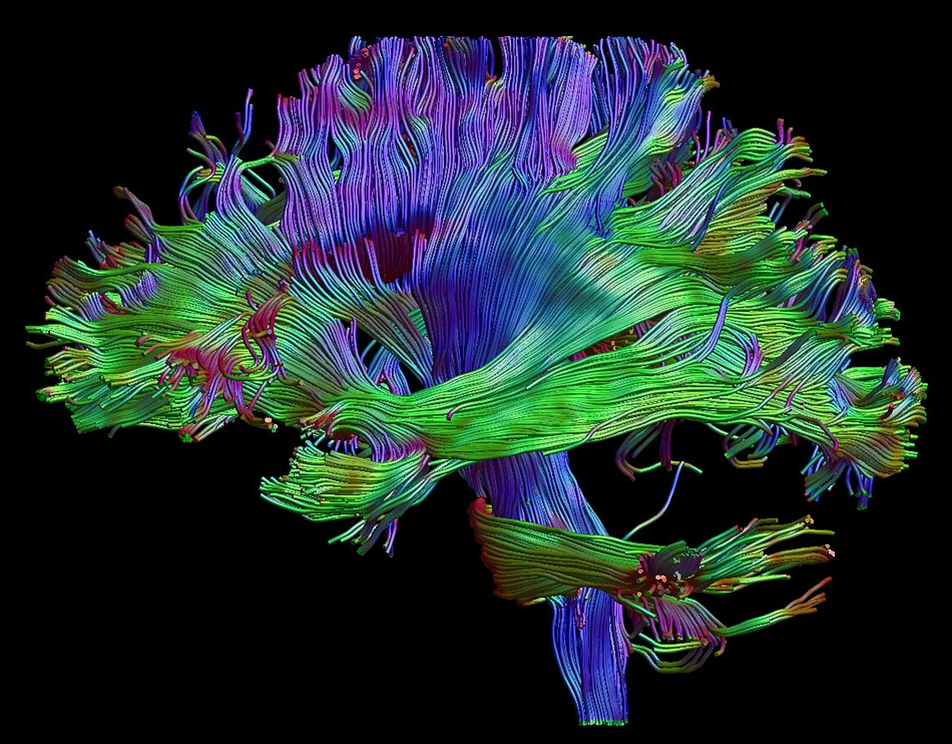
\includegraphics[width=.8\textwidth]{img/brain.png}
\end{center}
\end{frame}

\begin{frame}[t]{MRI Evaluation}
\begin{center}
\includegraphics[width=\textwidth]{img/grppi-phardi.pdf}
\end{center}
\end{frame}

%\begin{frame}{Observaciones}
%\begin{itemize}
%  \item Impacto del patrón \textgood{farm}:
%    \begin{itemize}
%      \item El uso de \textgood{farm} en ambas etapas causa una mejora sustancial del rendimiento.
%        \begin{itemize}
%          \item Equilibrio.
%        \end{itemize}
%      \item El uso de \textgood{farm} en una única etapa del pipeline no tiene impacto significativo.
%        \begin{itemize}
%          \item Desequilibrio.
%        \end{itemize}
%    \end{itemize}
%
%  \vfill\pause
%  \item Impacto de GrPPI en el rendimento.
%    \begin{itemize}
%      \item Sobrecoste por debajo del 2\%.
%    \end{itemize}
%
%  \vfill\pause
%  \item Impacto en el esfuerzo.
%    \begin{itemize}
%      \item Reducción significativa con respecto a los otros enfoques de programación.
%    \end{itemize}
%\end{itemize}
%\end{frame}
%
%\begin{frame}[t]{Conclusiones}
%\begin{itemize}
%  \item GrPPI permite cambiar de modelo de programación subyacente con mínimo esfuerzo
%        gracias al uso de C++ moderno.
%  \vfill\pause
%  \item Diseño compacto para ocultar la complejidad de alternativas de implementación.
%  \vfill\pause
%  \item Soporte de múltiples patrones:
%    \begin{itemize}
%      \item \textenum{Datos/}: \textmark{map}, \textmark{reduce}, \textmark{map/reduce}, \textmark{stencil}.
%      \item \textenum{Tareas}: \textmark{divide/conquer}.
%      \item \textenum{streaming} \textmark{pipeline} con etapas \textmark{farm}, \textmark{filter}, \textmark{reduce},
%                                 \textmark{iteration}.
%    \end{itemize}
%  \vfill\pause
%  \item Mínimo sobrecoste de:
%    \begin{itemize}
%      \item Modificaciones del código fuente.
%      \item Rendimiento.
%    \end{itemize}
%\end{itemize}
%\end{frame}
%
%\begin{frame}[t]{Trabajo futuro}
%\begin{itemize}
%  \item Mejorar y ampliar políticas de ejecución (Thrust, FastFlow, \ldots).
%  \item Incorporar nuevos patrones.
%  \item Extender y simplificar la interfaz para patrones de datos.
%  \item Dar soporte a combinación de políticas de ejecución.
%  \item Mejorar el soporte NUMA.
%  \item Ampliar aplicaciones ejemplo y benchmarks.
%  \vfill
%  \item \textgood{\url{https:/www.github.com/arcosuc3m/grppi}}.
%\end{itemize}
%\end{frame}
